\documentclass{article}
\usepackage{amsmath}
\usepackage{amsfonts}
\usepackage{amssymb}
\usepackage{amsthm}
\usepackage{geometry}
\usepackage{algorithm}
\usepackage{algpseudocode}
\usepackage{minted}
\usepackage{graphicx}
\usepackage{booktabs} % For professional tables
\usepackage{caption}

\geometry{a4paper, left=2cm, right=2cm, top=2cm, bottom=2cm}

\title{Report for AI Capstone Homework 2: 3D Scene Reconstruction}
\author{FU, YONG-WEI (112550107)}
\date{\today}

\begin{document}
\sloppy

\maketitle

\section{Implementation}

\subsection{Code: Pipeline Explanation}
The 3D scene reconstruction pipeline was implemented using Python, NumPy, and Open3D. 
Below is a detailed breakdown of the techniques and algorithms used in each stage:

\begin{enumerate}
    \item \textbf{Data Collection, Loading \& Depth Quantization Fix:} 
    $load.py$ was first used to traverse the room and collect the rgb, depth, and semantic images.
    Later on, $reconstruct.py$ was used to load the collected data and to reconstruct the 3D scene in point cloud format. 
    The code was modified to preserve the depth information (maximum 10 meters) as a 16-bit unsigned integer, rather than 
    as a 8-bit integer. This preserved accuracy and adhered to the specification's \texttt{DEPTH\_SCALE = 1000.0}. 
    The ground truth trajectory was also loaded into the process here.

    \item \textbf{Unprojection:}
    Took the first image and used the depth information to unproject the rgb points into 3D space in point cloud format. 

    \item \textbf{Pre-processing:}
    Applied Voxel Downsampling to reduce the point count. Later, calculated the normal vectors of the 
    points, so that the Fast Point Feature Histograms (FPFH) can extract local geometric features for 
    each point, which will be later used to align the point clouds.

    \item \textbf{Registration:}
    \begin{itemize}
        \item \textbf{Global Registration (RANSAC):}
        After obtaining the FPFH features of two point clouds with the procedure above, RANSAC was used to roughly align the latter point cloud to the previous one.
        I utilized a high iteration count (up to 1.5M) to ensure a better probability of success.
        \item \textbf{Local Registration (ICP):}
        Used Point-to-Plane ICP to refine the RANSAC result by minimizing the distance between corresponding points. 
        Lastly, add them to the accumulated point cloud, store the new camera pose (by multiplying the previous pose with the estimated transformation) and 
        repeat the process until the end of the collected data.
    \end{itemize}

    \item \textbf{Post-processing (Ceiling Removal):}
    Implemented a height-based mask to remove the ceiling for visualization. 
    This is integrated into the evaluation phase rather than the reconstruction phase to maintain the geometric integrity of the raw data.
\end{enumerate}

\subsection{Result \& Discussion}

\subsubsection{Screenshots}
\begin{figure}[H]
    \centering
    % Row 1
    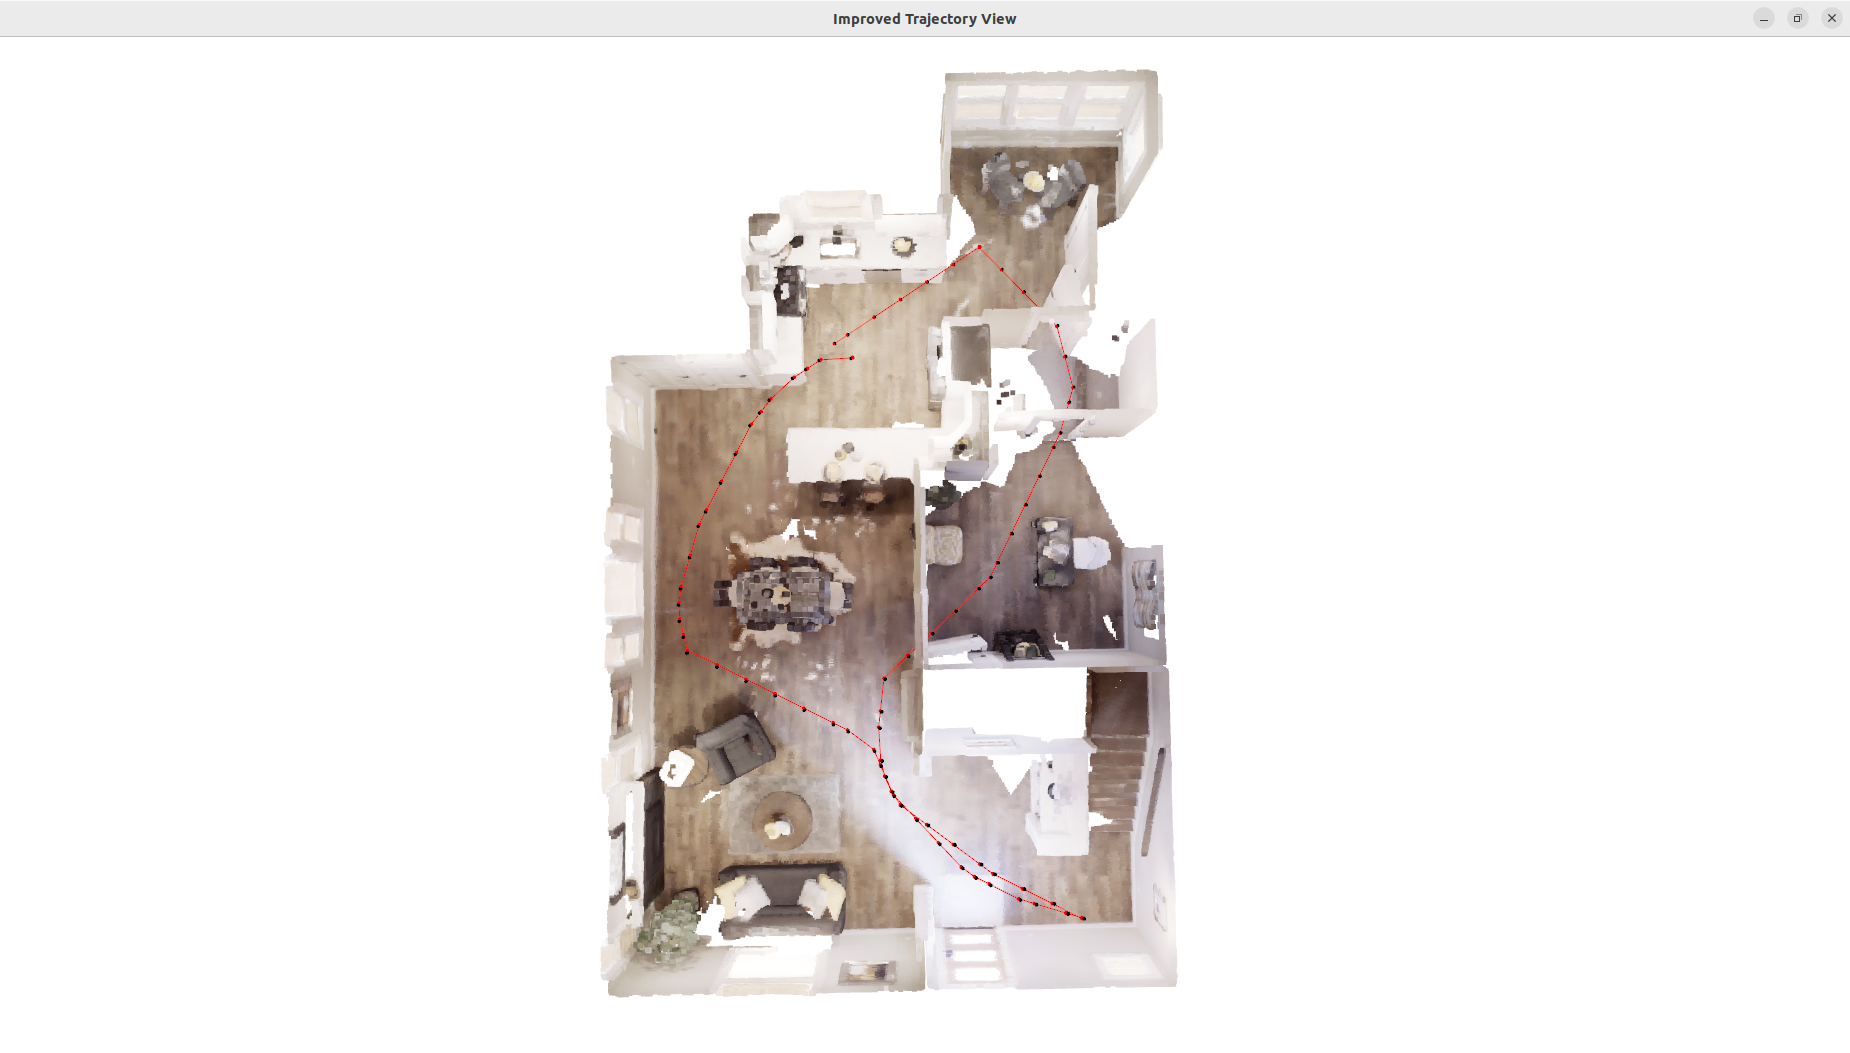
\includegraphics[width=0.4\textwidth]{screenshots/first_1.png}
    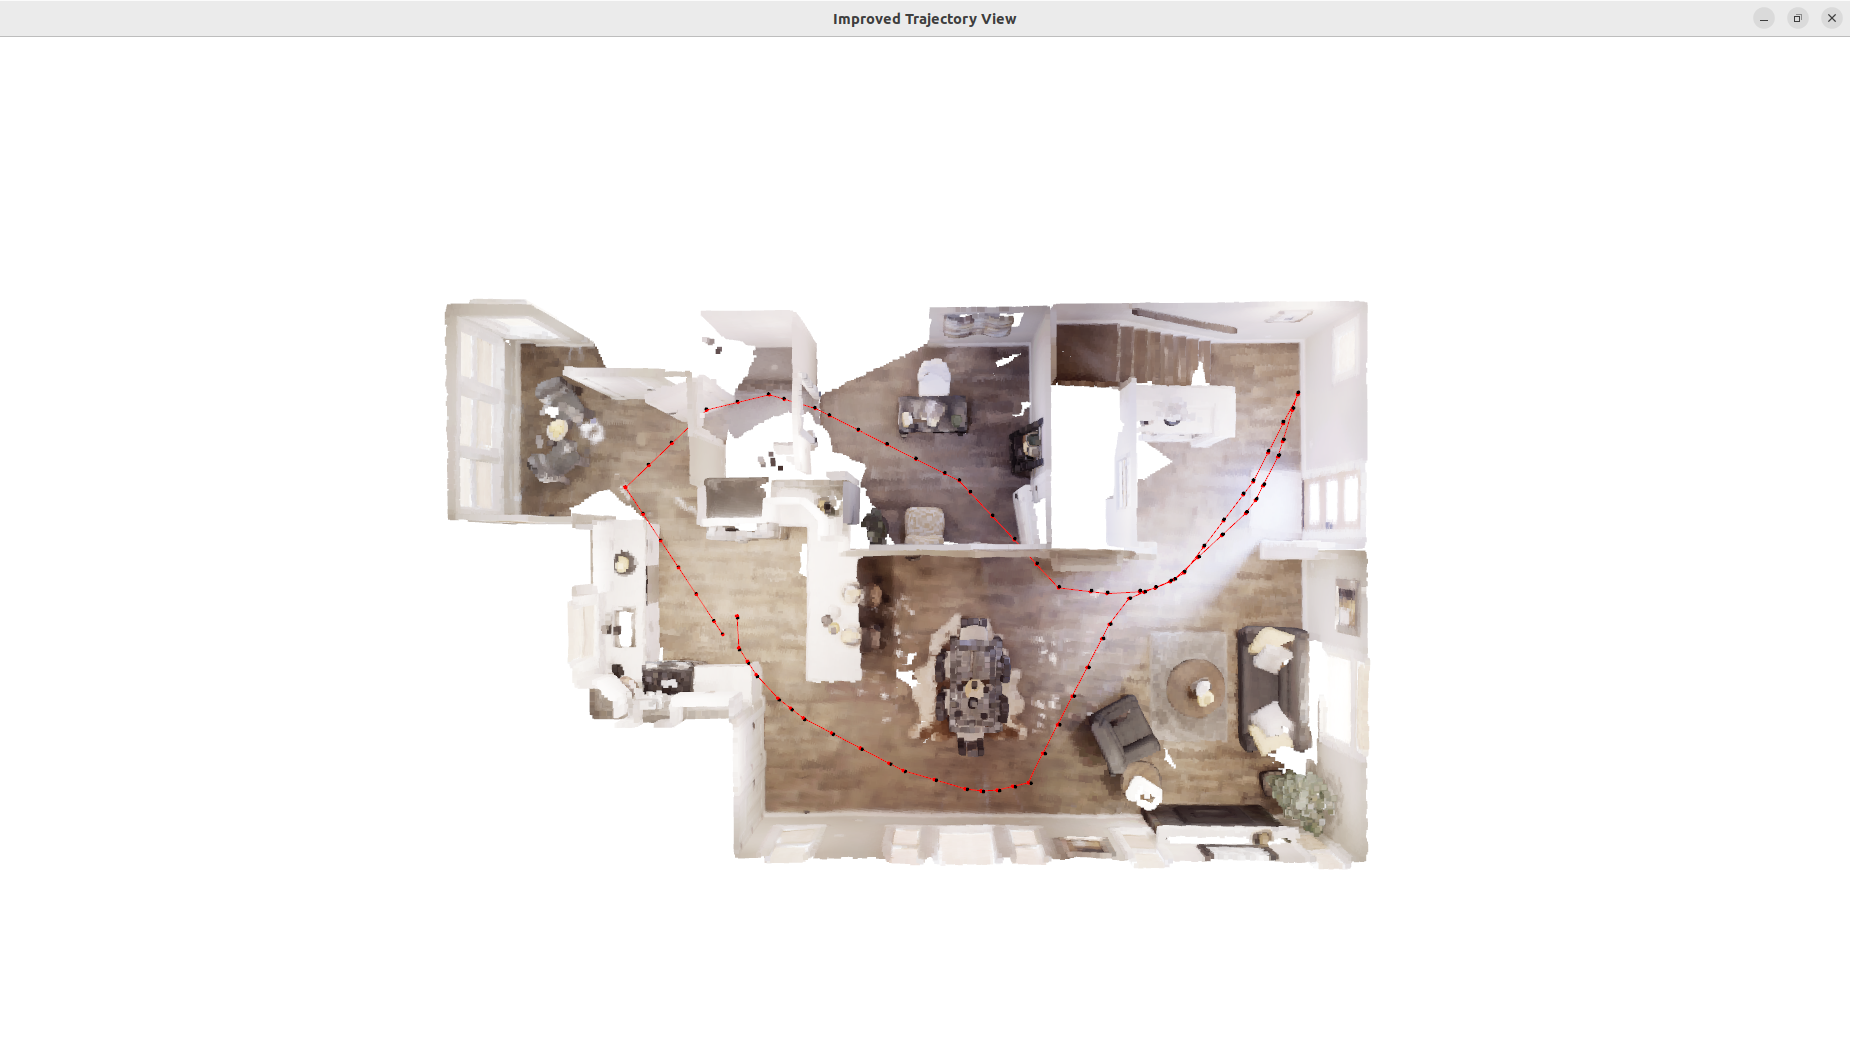
\includegraphics[width=0.4\textwidth]{screenshots/first_2.png}
    \\[0.5cm] % Adds a little vertical space between rows
    % Row 2
    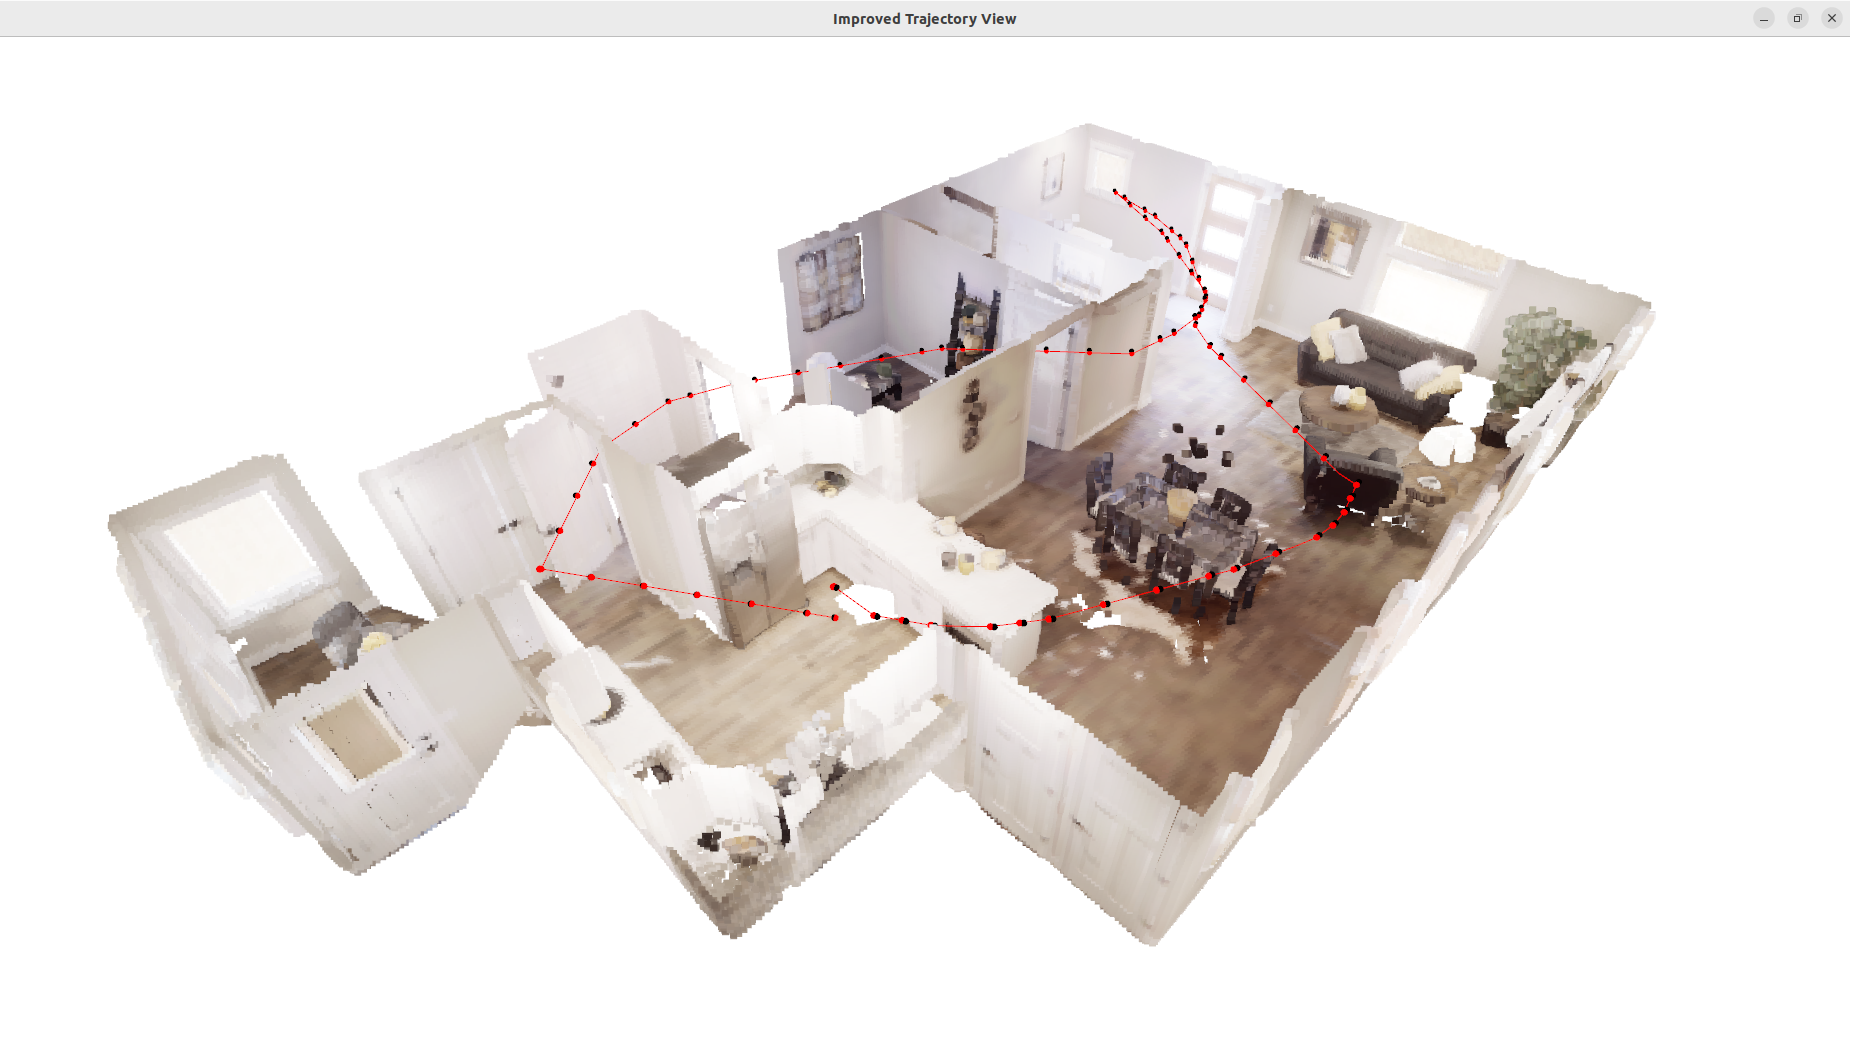
\includegraphics[width=0.4\textwidth]{screenshots/first_3.png}
    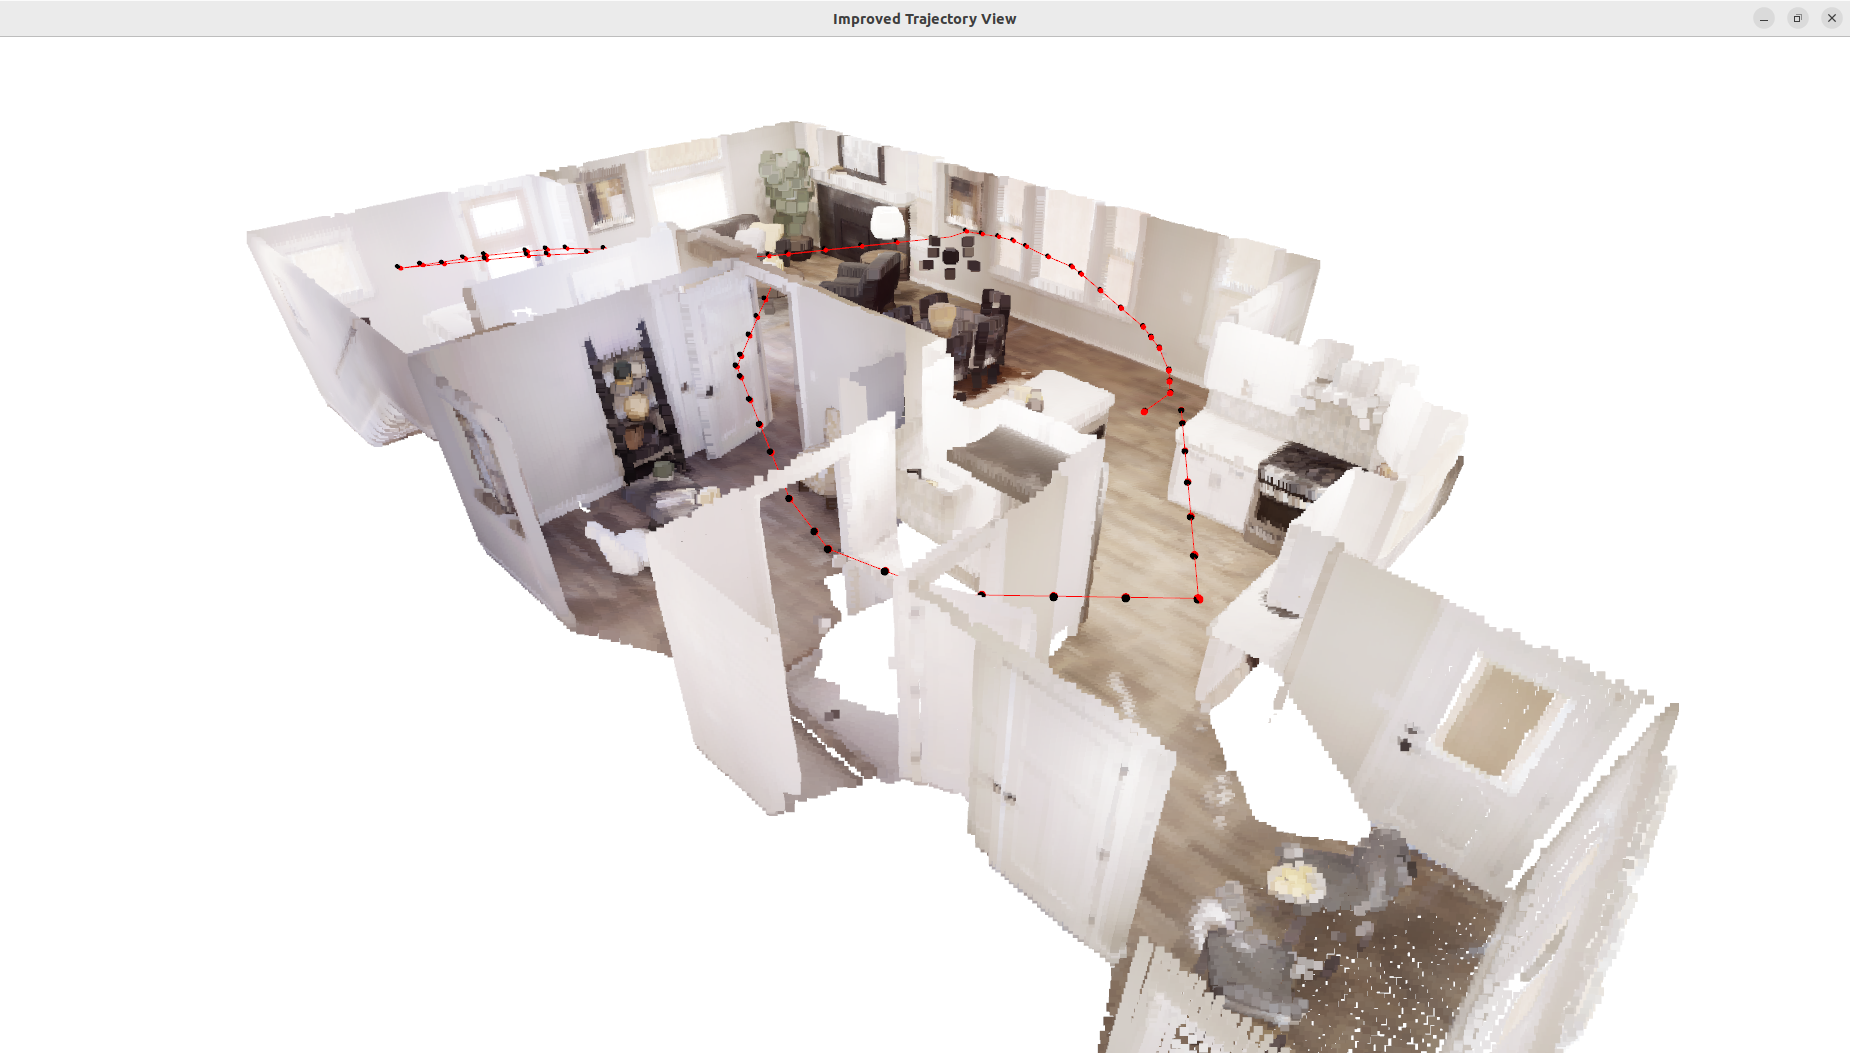
\includegraphics[width=0.4\textwidth]{screenshots/first_5.png}
    \\[0.5cm] % Adds a little vertical space between rows
    % Row 3
    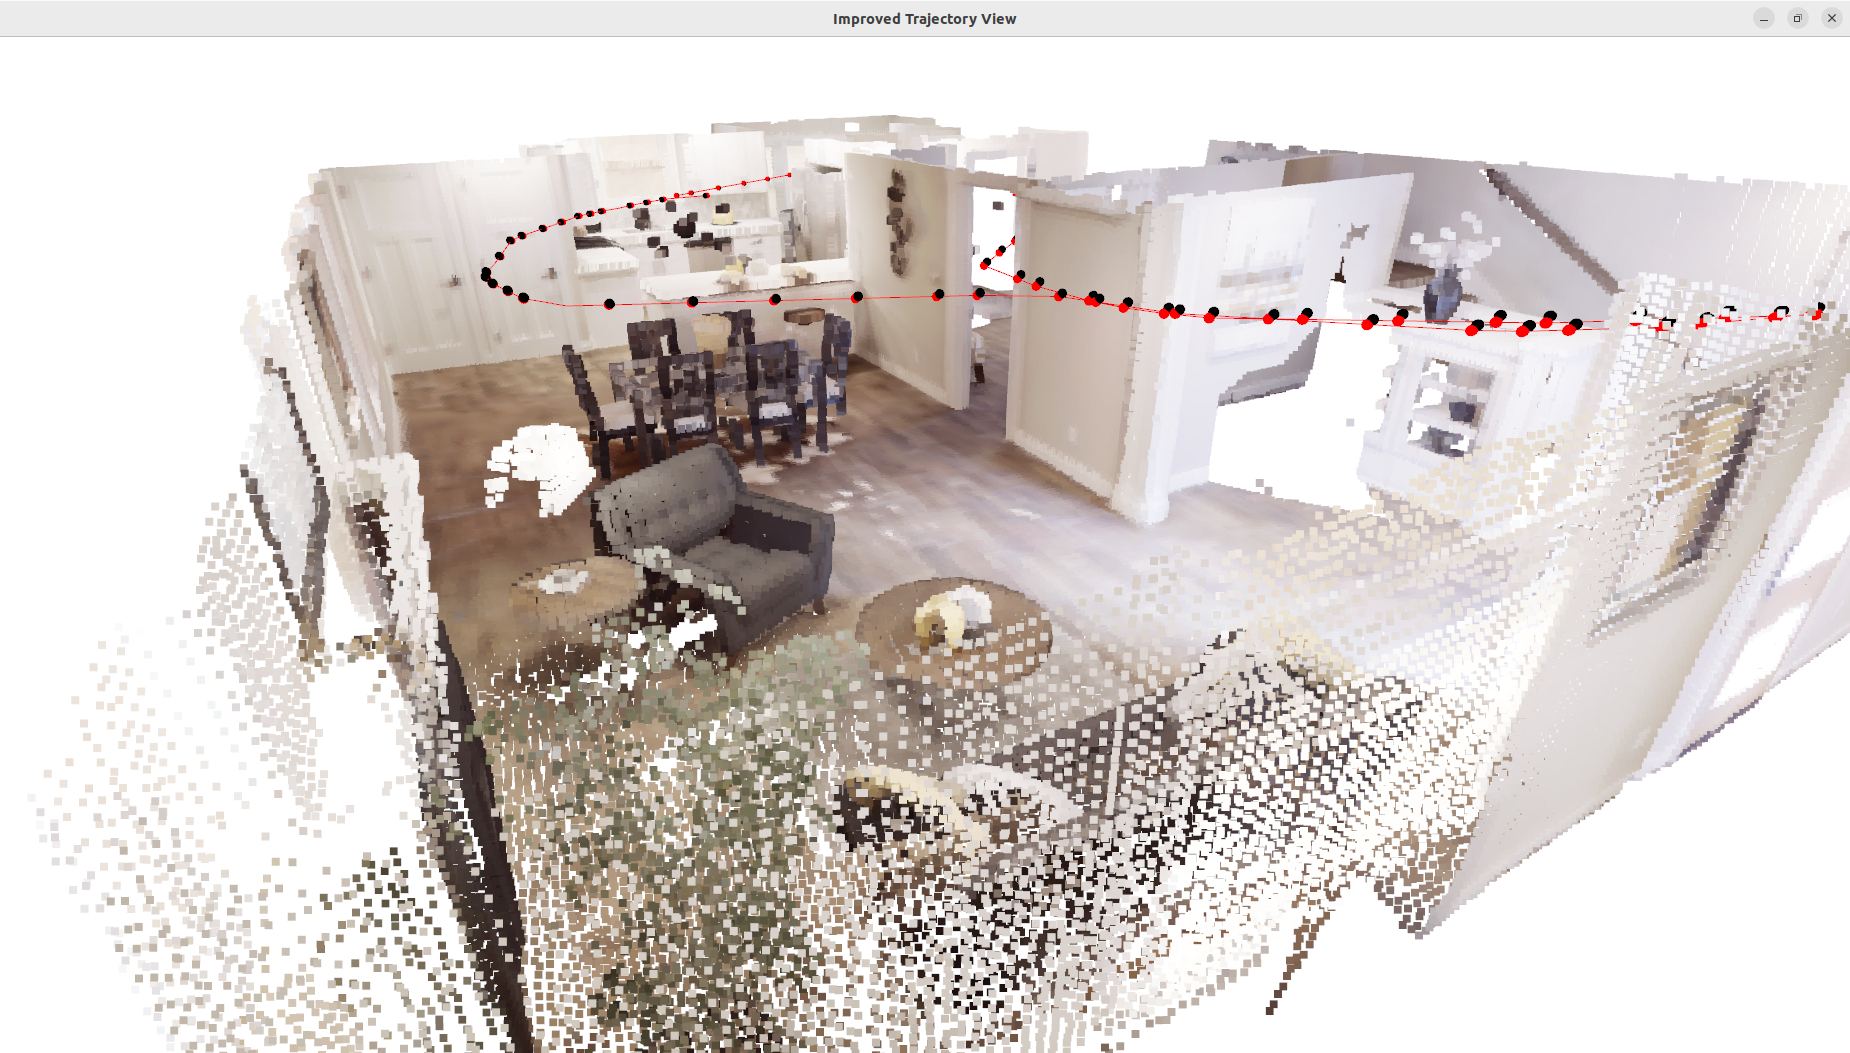
\includegraphics[width=0.4\textwidth]{screenshots/first_4.png}
    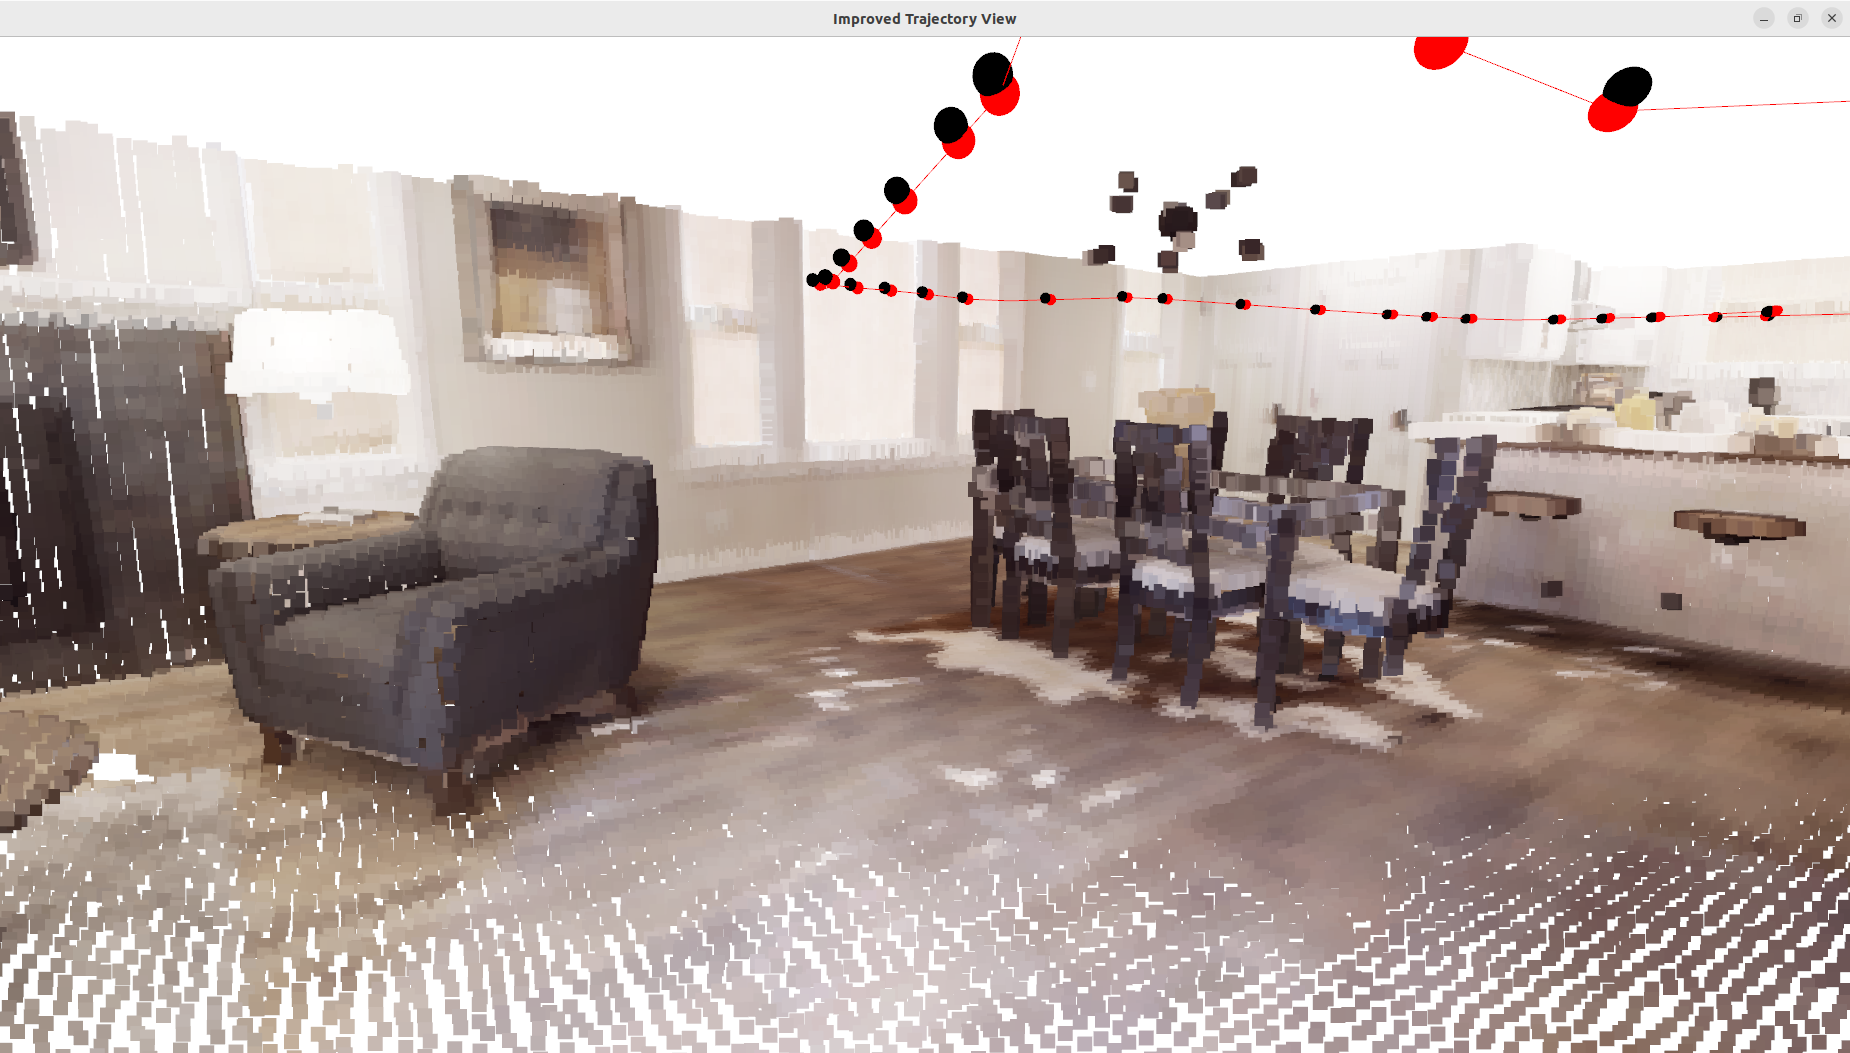
\includegraphics[width=0.4\textwidth]{screenshots/first_6.png}
    
    \caption{Floor 1 Reconstruction Overview: (Top) Bird's-eye views of apartment\_0; (Middle) Side views; (Bottom) Close-up view.}
    \label{fig:floor1}
\end{figure}

\subsubsection{Comparison Table}
The following table summarizes the hyperparameter search conducted to optimize 
for both Mean L2 Error and execution time. (the experiment were run on the second floor.)

\begin{table}[H]
    \centering
    \resizebox{\textwidth}{!}{
        \begin{tabular}{@{}clccccccc@{}}
            \toprule
                \textbf{Exp \#} & \textbf{Voxel (m)} & \textbf{RANSAC Iter} & \textbf{RANSAC Thresh / Voxel} & \textbf{FPFH max\_nn} & \textbf{Total Points} & \textbf{Mean L2 (m)} & \textbf{Time (s)} \\ \midrule
                0 & 0.04 & 1,500,000 & 2.5 & 100 & 196,933 & \textbf{0.038497} & 81.39 \\
                1 & 0.04 & 1,500,000 & 0.1 & 100 & 185,894 & 0.130952 & 176.67 \\
                2 & 0.08 & 1,500,000 & 0.2 & 100 & 54,812 & 0.201518 & \textbf{53.00} \\
                3 & 0.04 & 100,000 & 0.1 & 100 & 180,029 & 0.198384 & 80.77 \\
                4 & 0.04 & 1,500,000 & 0.048 & 100 & 177,681 & 0.130922 & 224.23 \\
                5 & 0.04 & 1,500,000 & 0.1 & 50 & 197,248 & 0.038534 & 188.64 \\
            \bottomrule
        \end{tabular}
    }
    \caption{Hyperparameter tuning, trajectory error, and execution time.}
    \label{tab:results}
\end{table}

\subsubsection{Discussion \& Findings}
Based on the experimental results, several key insights were identified:

\begin{itemize}
    \item \textbf{The Iteration Bottleneck (Exp 3):} Reducing RANSAC iterations from 1.5M to 100k caused the Mean L2 Error to jump significantly (from 0.038m to 0.198m). 
    Because the agent's step size in Habitat is 0.25m, the inadequate steps would lead to a extremely low inlier ratio. 
    Therefore, we can see that the stochastic nature of RANSAC requires a higher ``search budget'' to find the correct transformation; otherwise, it converges to local minima.
    \item \textbf{Voxel Trade-offs (Exp 2):} Increasing the voxel size to 0.08m achieved the fastest execution time (53s), but significant cost to accuracy was incurred. 
    The coarse geometry makes it difficult for Point-to-Plane ICP to calculate accurate normals, leading to increased odometry drift.
    \item \textbf{RANSAC Thresholding (Exp 4):} This experiment demonstrated that a tight RANSAC threshold ($0.048 \times 0.04 = 0.00192 \simeq 2\text{ mm}$) makes the system less 
    robust to Habitat's discrete movement. If the threshold is smaller than the noise or the actual jump between frames, RANSAC fails to identify valid correspondences, leading to 
    higher error and awful trajectory estimation.
    \item \textbf{Feature Optimization (Exp 5):} Reducing the FPFH nearest neighbors to 50 maintained high accuracy (0.038m). This suggests that for indoor environments with many planar surfaces, local geometric signatures do not require high neighbor density to remain descriptive.
\end{itemize}

\section{Questions}

\subsection{What happens if you perform ICP without Global Registration (RANSAC)? Why?}
If standard ICP is performed without an initial coarse alignment from RANSAC, the algorithm will frequently fail or 
converge into a local minimum. I would say that ICP is ``taking small but concise steps'', where RANSAC is ``taking big but noisy steps''. 
It is merely a local optimization algorithm, therefore it's nearly impossible to achieve global convergence without a good initial guess. 
To obtain that initial guess, RANSAC is thus put into use before ICP.

\subsection{Describe any tricks used to improve your ICP stability.}
% \begin{itemize}
%     \item \textbf{Point-to-Plane Estimation:} In geometric indoor environments, Point-to-Plane ICP allows the current frame to mathematically slide along planar surfaces (walls/floors), preventing the "stuck" behavior often seen in Point-to-Point estimation.
%     \item \textbf{Voxel-Based Normal Estimation:} Using a radius-based normal estimation (2x voxel size) ensures that even with downsampled data, the underlying surface geometry is accurately represented.
%     \item \textbf{Trajectory Visualization:} Representing camera poses as 3D spheres rather than just lines allowed for easier identification of "jumps" or "teleportation" errors during the tuning process.
% \end{itemize}

\end{document}

% odometry drift: i thought the ceiling is monotonic increasing or someshit
% why it doubled: look at 0408232714, also at that time, both the RANSAC and ICP inliers are low as fuck, it's because the voxel size is too big and had the wrong proportion for both thresholds